%%% Início dos anexos ------------------------------------------------
\anexos

\partanexos*

\chapter{Algoritmo de recomendação}

\section{Filtragem Colaborativa}

\subsection{Estruturação dos dados}

Inicialmente é necessário organizar os dados existentes para a realização da recomendação. Para isso, é gerado um tabela que demonstra as notas avaliadas pelos avaliadores para os itens no sistema, conforme mostrado na figura \ref{fig:avaliacoes}. Os campos em amarelo representam os valores ainda não avaliados, sendo tarefa do sistema de recomendação calcular as possíveis notas dos avaliadores para esses campos.

\begin{figure}[H]
	\centering
	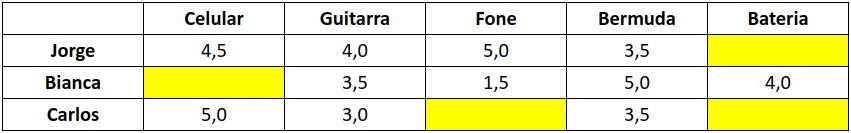
\includegraphics[width=0.8\linewidth]{imagens/recomendacaoAvaliacoes.jpg}
	\caption[Avaliações dos itens pelos avaliadores]{Avaliações dos itens pelos avaliadores}
    \label{fig:avaliacoes}
\end{figure}

\subsection{Similaridade entre os avaliadores}

Como a recomendação colaborativa usa como base o conceito de vizinhança para seus cálculos, é necessário medir a distância existente entre os avaliadores. Para esse exemplo será usado o cálculo da distância do avaliador Jorge em relação a todos os outros avaliadores do sistema, conforme mostrado na figura \ref{fig:similaridadeJorge}. De maneira geral, esse processo deverá ser realizado para todos os avaliadores do sistema.

\begin{figure}[H]
	\centering
	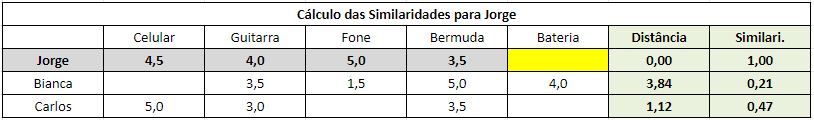
\includegraphics[width=1\linewidth]{imagens/similaridadeJorge.png}
	\caption[Cálculo da similaridade do Jorge com os avaliadores]{Cálculo da similaridade do Jorge com os avaliadores}
    \label{fig:similaridadeJorge}
\end{figure}

Para esse cálculo foi utilizado a fórmula da distância euclidiana, utilizando como parâmetros as notas informadas pelos avaliadores em cada um dos itens. Para cálculo da distância euclidiana é utilizado um conjunto de pares, representado pela notas de Jorge e do avaliador calculado no momento acerca de determinado item. Caso algum dos parâmetros esteja vazio, a coordenada é ignorada pelo algoritmo no cálculo da distância.

Para facilitar a visualização o cálculo da distância euclidiana foi decomposto nos seguintes passos:

\begin{itemize}
    \item Definição das coordenadas;
    \item Cálculo do quadrado da diferença;
    \item Somatório dos quadrados da diferença;
    \item Raiz quadrado do somatório dos quadrados da diferença.
\end{itemize}

Nos cálculos abaixo, é possível observar a geração da distância euclidiana entre Jorge e Bianca:

\subsubsection{Definição das coordenadas}

Separando as coordenadas válidas obteremos uma tabela conforme demonstrado na figura \ref{fig:coordenadasEuclidiana}:

\begin{figure}[H]
	\centering
	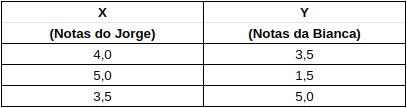
\includegraphics[width=.7\linewidth]{imagens/coordenadasEuclidiana.jpg}
	\caption[Coordenadas para distância euclidiana]{Coordenadas para distância euclidiana entre Jorge e Bianca}
    \label{fig:coordenadasEuclidiana}
\end{figure}

\subsubsection{Cálculo do quadrado da diferença}

Aplicando a fórmula do quadrado da diferença nas coordenadas apresentadas na figura \ref{fig:coordenadasEuclidiana} é possível chegar nos resultados descritos na figura \ref{fig:quadradoDiferenca}:

\begin{equation*}
    {F(x,y) = \left( x_{i}-y_{i}\right)^2 }
    \label{eq:quadradoDiferenca}
\end{equation*}

\begin{figure}[H]
	\centering
	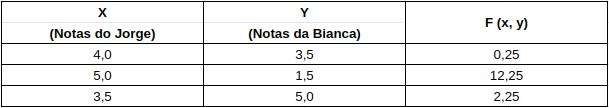
\includegraphics[width=.8\linewidth]{imagens/quadradoDiferenca.jpg}
	\caption[Quadrado da diferença das coordenadas]{Quadrado da diferença das coordenadas}
    \label{fig:quadradoDiferenca}
\end{figure}

\subsubsection{Somatório dos quadrados da diferença}

Nessa etapa, somente é necessário realizar a soma entre os dados encontrados na função \textbf{F(x)} mostrada na figura \ref{fig:quadradoDiferenca}. Desse modo chega-se na seguinte equação \ref{eq:somaQuadrados}:

\begin{equation*}
    \begin{aligned}
    {S(x,y)& = 0.25 + 12.25 + 2.25} \\
    {S(x,y)& = 14.75}
    \end{aligned}
    \label{eq:somaQuadrados}
\end{equation*}

\subsubsection{Raiz quadrado do somatório dos quadrados da diferença}

Aplicando a raiz quadrado sobre o resultado do somatório obtido na equação \ref{eq:somaQuadrados} obtemos o seguinte resultado apresentado na equação \ref{eq:raizSomaQuadrados}:

\begin{equation*}
    \begin{aligned}
    {D(x,y)& = \sqrt{S(x, y)} \\
    {D(x,y)& = \sqrt{14.75}} \\
    {D(x,y)& \approx{3.84}
    \end{aligned}
    \label{eq:raizSomaQuadrados}
\end{equation*}

A partir desses resultados é possível obter um coeficiente de distância entre o usuário Jorge e Bianca de aproximadamente \textbf{3.84}. A partir desse valor, é possível realizar a análise de distância entre todos os usuários do sistema e definir os vizinhos, que seriam os que apresentarem menor coeficiente de distância.

Para facilitar a visualização da distância também pode ser definido um coeficiente de similaridade, que poderia ser representado com a equação \ref{eq:similaridade} mostrada abaixo:

\begin{equation*}
    \begin{aligned}
    {Sm(x,y)& = 1/(1 + D(x,y))} \\
    {Sm(x,y)& = 1/1 + 3.84}} \\
    {Sm(x,y)& \approx{0.21}
    \end{aligned}
    \label{eq:similaridade}
\end{equation*}

Com o coeficiente de similaridade definido, podemos visualizar que quando maior esse valor, maior será a proximidade entre os usuários.

\subsection{Similaridade entre itens}

Com os coeficientes de similaridade definidos, pode-se calcular as notas dos itens para recomendação. Na abordagem colaborativa a similaridade dos usuários será utilizada como forma de peso para as suas avaliações, sendo que quanto mais próximo os usuários estejam, maior será o impacto de suas avaliações na nota que será recomendada pelo sistema.

Levando a análise do Jorge como exemplo, pode-se calcular as notas avaliadas pelos outros usuários acerca dos itens. Para isso, é realizado a multiplicação entre as notas avaliadas e o coeficiente de similaridade entre Jorge e o usuário em questão, conforme mostrado na figura \ref{fig:similaridadeAvaliacoes}:

\begin{figure}[H]
	\centering
	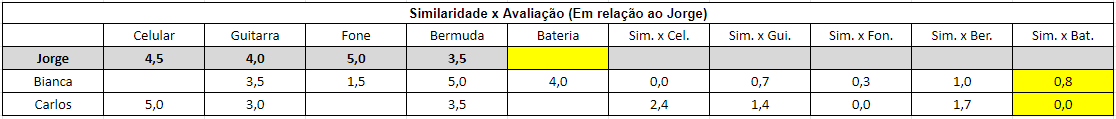
\includegraphics[width=1\linewidth]{imagens/similaridadeAvaliacao.PNG}
	\caption[Similaridade x Avaliações]{Similaridade x Avaliações}
    \label{fig:similaridadeAvaliacoes}
\end{figure}

\subsection{Cálculo da recomendação}

Com os dados de similaridade de itens disponíveis, é possível calcular a possível nota que o usuário dará para os itens que ainda não avaliou. Utilizando o exemplo do Jorge, é possível visualizar que a bateria ainda não foi avaliada. Dessa forma, pode-se calcular essa nota, utilizando os seguintes passos:

\begin{itemize}
    \item Soma das similaridades dos usuários;
    \item Soma das similaridades dos itens;
    \item Cálculo da recomendação.
\end{itemize}

\subsubsection{Soma das similaridades dos usuários}

Para realização dessa conta basta selecionar todos os usuários que avaliaram o item que será recomendado (no exemplo do Jorge, a bateria) e somar o valor de suas similaridades, conforme a equação \ref{eq:somatorioSimilaridadeUsuarios}:

\begin{equation*}
    \begin{aligned}
    {Su(x,y)& = 0.21}
    \end{aligned}
    \label{eq:somatorioSimilaridadeUsuarios}
\end{equation*}

\textbf{OBS:} Como Carlos não avaliou a bateria sua nota será desconsiderada nesse cálculo.

\subsubsection{Soma das similaridades dos itens}

Nessa etapa. deve-se realizar o somatório de todos as avaliações do item que será recomendado. No exemplo utilizado, usaremos somente a nota da Bianca acerca da bateria, uma vez que o Carlos não avaliou esse item. Com isso, chegamos na equação \ref{eq:somatorioSimilaridadeUsuarios}:

\begin{equation*}
    \begin{aligned}
    {Si(x,y)& = 0.8}
    \end{aligned}
    \label{eq:somatorioSimilaridadeUsuarios}
\end{equation*}

\subsubsection{Cálculo da recomendação}

Com os somatórios das similaridades realizados, basta realizar uma divisão entre seus valores, conforme mostrado na equação \ref{eq:calculoRecomendacaoColaborativa} para se obter o valor da recomendação do item.

\begin{equation*}
    \begin{aligned}
    {R(x,y)& = Si/Su} \\
    {R(x,y)& = 0.8/0.21}
    {R(x,y)& = 3.8}
    \end{aligned}
    \label{eq:calculoRecomendacaoColaborativa}
\end{equation*}

Com isso podemos definir que a nota gerada pelo sistema para bateria ao Jorge será de \textbf{3.8}.

\section{FILTRAGEM BASEADA EM CONTEÚDO}

\subsection{Estruturação dos dados}

A organização dos dados iniciais para filtragem baseada em conteúdo pode ser dividida em duas partes, sendo uma da relação entre os avaliadores e os itens (igual a utilizada na filtragem colaborativa) e outra que apresenta os vínculos entre os itens e as tags. Ambas as tabelas podem ser visualizadas nas figuras \ref{fig:avaliacoes2} e \ref{fig:itensTags}:

\begin{figure}[H]
	\centering
	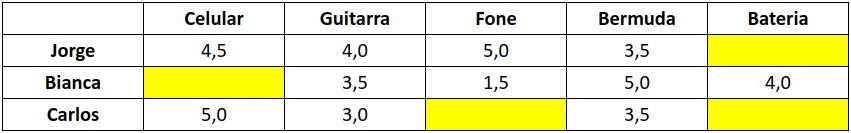
\includegraphics[width=.8\linewidth]{imagens/recomendacaoAvaliacoes.jpg}
	\caption[Avaliações dos itens pelos avaliadores]{Avaliações dos itens pelos avaliadores}
    \label{fig:avaliacoes2}
\end{figure}

\begin{figure}[H]
	\centering
	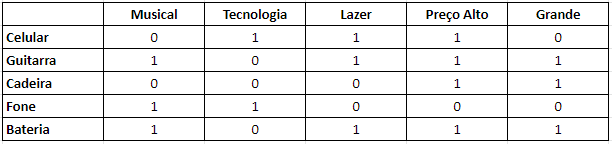
\includegraphics[width=.8\linewidth]{imagens/itemTags.PNG}
	\caption[Itens x Tags]{Itens x Tags}
    \label{fig:itensTags}
\end{figure}

\subsection{Identificação dos Perfis}

Na filtragem baseada em conteúdo têm-se como principal alvo o uso das características dos itens para geração da recomendação. Para isso, necessita-se criar e avaliar qual o impacto de cada tag para o usuário avaliado.

Para essa avaliação, será realizado a criação de perfil para o usuário. Usando o exemplo do Jorge, pode-se chegar no perfil apresentado na figura \ref{fig:perfilUsuario} a partir da multiplicação da nota avaliada pelo usuário e a relação entre item e tag existente para cada item. Vale ressaltar que nas duas últimas linhas da tabela exibida na figura \ref{fig:perfilUsuario} têm-se o somatório e média de cada tag.

\begin{figure}[H]
	\centering
	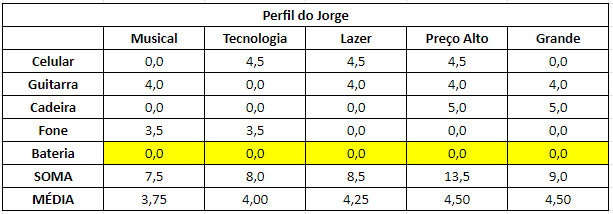
\includegraphics[width=.8\linewidth]{imagens/perfilUsuario.PNG}
	\caption[Perfil do Jorge]{Perfil do Jorge}
    \label{fig:perfilUsuario}
\end{figure}

\subsection{Similaridade entre as tags}

Para definir a similaridade dos itens com o usuário é necessário a utilização do perfil criado no passo anterior. Para definição dos coeficientes é necessário realizar o cálculo da distância euclidiana entre as notas avaliadas pelo usuário e os valores calculados para seu perfil. Para exemplificação, pode-se analisar a figura \ref{fig:coordenadasConteudo} que mostra o cálculo da distância euclidiana entre Jorge e o Celular:

\begin{figure}[H]
	\centering
	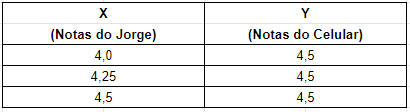
\includegraphics[width=.8\linewidth]{imagens/coordenadasConteudo.PNG}
	\caption[Coordenadas para distância euclidiana]{Coordenadas para distância euclidiana}
    \label{fig:coordenadasConteudo}
\end{figure}

Após realização dos cálculos pode-se obter o coeficiente de similaridade entre Jorge e os itens, conforme mostrado na figura \ref{fig:similaridadeConteudo}. Vale ressaltar que os cálculos de distância euclidiana e coeficiente de similaridade são os mesmos apresentados na seção de filtragem colaborativa, apenas mudando as variáveis comparadas. 

\begin{figure}[H]
	\centering
	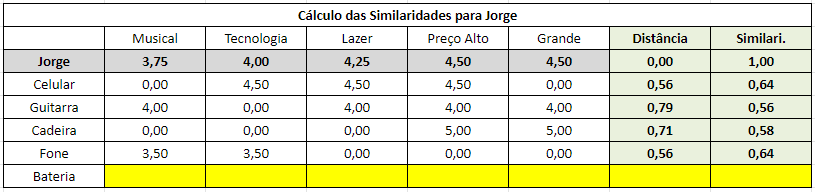
\includegraphics[width=1\linewidth]{imagens/similaridadeConteudo.PNG}
	\caption[Similaridade de Itens com Jorge]{Similaridade de Itens com Jorge}
    \label{fig:similaridadeConteudo}
\end{figure}

\subsection{Similaridade entre os itens}

A partir da realização dos passos anteriores, é possível definir a similaridade dos itens multiplicando seu perfil com o valor de similaridade obtido na etapa anterior. Desse modo, é possível chegar no resultado mostrado na figura \ref{fig:similaridadeConteudoItem}:

\begin{figure}[H]
	\centering
	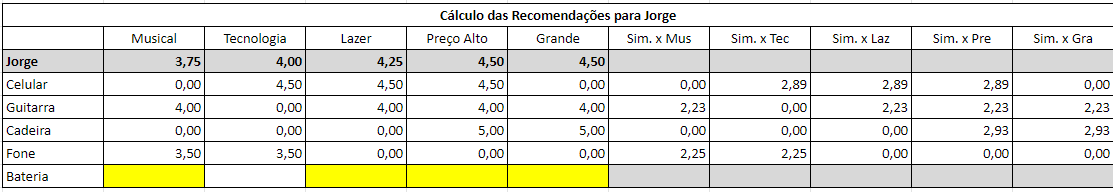
\includegraphics[width=1\linewidth]{imagens/similaridadeConteudoItem.PNG}
	\caption[Similaridade dos Itens com as tags]{Similaridade dos Itens com as tags}
    \label{fig:similaridadeConteudoItem}
\end{figure}

\subsection{Cálculo da nota das tags do Item}

Com a similaridade dos itens definida, é possível definir o peso das característica para os itens ainda não avaliados. Para isso, é necessário a realização dos seguintes passos:

\begin{itemize}
    \item Somatório das similaridades da tag avaliada;
    \item Somatório das similaridades dos itens que possuem a tag avaliada;
    \item Divisão dos somatórios das similaridades.
\end{itemize}

\subsubsection{Somatório das similaridades da tag avaliada}

Utilizando como base a tabela exibida na figura \ref{fig:similaridadeConteudoItem} pode-se exemplificar o somatório da tag \textbf{Musical}. Para isso, basta realizar o somatório da columa \textbf{Sim. x Mus}, como mostrado na equação abaixo:

\begin{equation*}
    \begin{aligned}
    {St(x,y)& = 0 + 2.23 + 0 + 2.23} \\
    {St(x,y)& = 4.46}
    \end{aligned}
    \label{eq:calculoRecomendacaoColaborativa}
\end{equation*}

\subsubsection{Somatório das similaridades dos itens que possuem a tag avaliada}

Para realização desse cálculo é necessário selecionar todos os itens tem vínculo com a tag analisada e realizar o somatório de sua similaridade. No exemplo será utilizada a tag \textbf{Musical}, fazendo com que sejam selecionados os itens \textbf{Guitarra} e \textbf{Fone}. O valor da similaridade está disponível no perfil do usuário e a conta realizada é mostrada na equação \ref{eq:somaSimilaridadeItem}:

\begin{equation*}
    \begin{aligned}
    {Sit(x,y)& = 0.56 + 0.64} \\
    {Sit(x,y)& = 1.2}
    \end{aligned}
    \label{eq:somaSimilaridadeItem}
\end{equation*}

\subsubsection{Divisão dos somatórios das similaridades}

Com os somatórios realizados nos itens anteriores, basta realizar o passo mostrado na equação \ref{eq:valorTagItem} para descobrir o valor da tag para o item que ainda não foi avaliado (no exemplo usado, a bateria).

\begin{equation*}
    \begin{aligned}
    {Vt(x,y)& = St(x,y)/Sit(x,y)} \\
    {Vt(x,y)& = 4.46/1.2} \\
    {Vt(x,y)& \approx{3.72}}
    \end{aligned}
    \label{eq:valorTagItem}
\end{equation*}

Desse modo, é possível definir o valor \textbf{3.72} para a tag \textbf{Musical} no item \textbf{Bateria}.

\subsection{Cálculo da recomendação}

Com a definição do valor de todas as tags para o item ainda não avaliado, conforme demonstrado na figura \ref{fig:notasTags}, basta realizar a média desses valores para obter a nota do item, conforme demonstrado na equação \ref{eq:mediaTags}:

\begin{figure}[H]
	\centering
	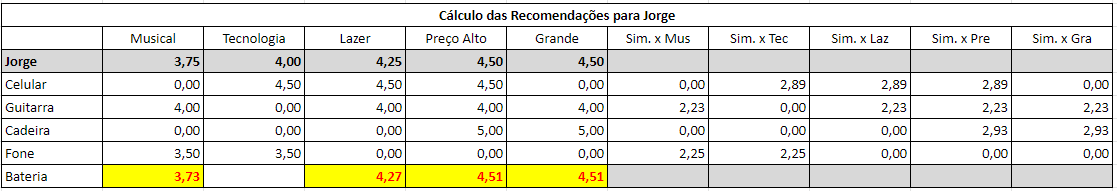
\includegraphics[width=1\linewidth]{imagens/notasTags.PNG}
	\caption[Notas das tags para bateria]{Notas das tags para bateria}
    \label{fig:notasTags}
\end{figure}

\begin{equation*}
    \begin{aligned}
    {R(x,y)& = (3.73 + 4.27 + 4.51 + 4.51)/4} \\
    {R(x,y)& = 17.02/4} \\
    {R(x,y)& \approx{4.25}}
    \end{aligned}
    \label{eq:mediaTags}
\end{equation*}

Dessa maneira o sistema pode recomendar o item \textbf{Bateria} com a nota \textbf{4.25}.